% Cover
\imprimircapa

% False cover sheet
%\imprimirfalsafolhaderosto

% Cover sheet
\imprimirfolhaderosto

% Card Catalog
\begin{fichacatalografica}
	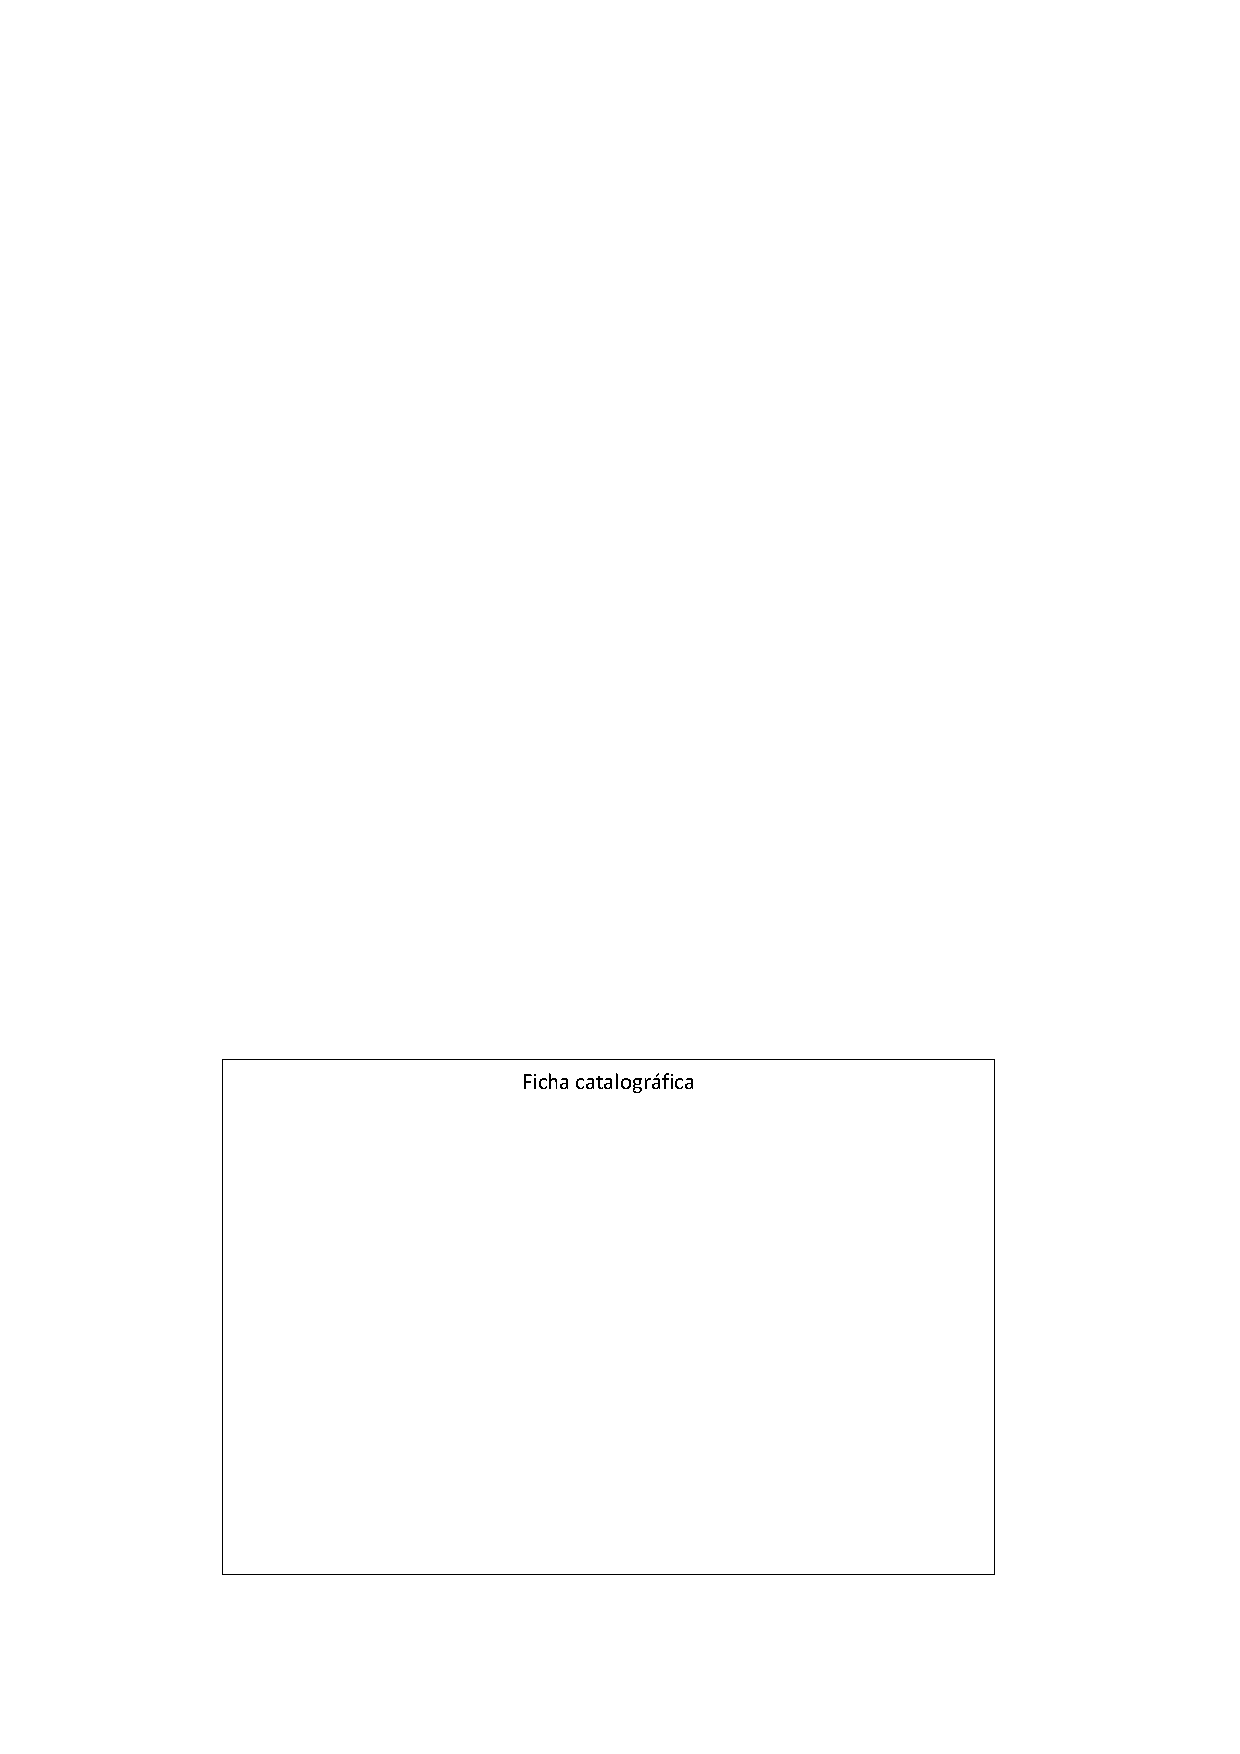
\includepdf{card-catalog.pdf}
\end{fichacatalografica}

% Approval sheet
%\begin{folhadeaprovacao}
%	
%	\begin{center}
%		{\ABNTEXchapterfont\large\imprimirautor}
%		
%		\vspace*{\fill}\vspace*{\fill}
%		\begin{center}
%			\ABNTEXchapterfont\bfseries\Large\imprimirtitulo
%		\end{center}
%		\vspace*{\fill}
%		
%		\hspace{.45\textwidth}
%		\begin{minipage}{.5\textwidth}
%			\imprimirpreambulo
%		\end{minipage}%
%		\vspace*{\fill}
%	\end{center}
%	
%	%Trabalho aprovado. \imprimirlocal, 31 de dezembro de 2020:
%	
%	\assinatura{\textbf{\imprimirorientador} \\ Orientador} 
%	\assinatura{\textbf{\imprimircoorientador} \\ Coorientador} 
%	\assinatura{\textbf{A} \\ Convidado 1}
%	\assinatura{\textbf{B} \\ Convidado 2}
%	
%	\begin{center}
%		\vspace*{0.5cm}
%		{\large\imprimirlocal}
%		\par
%		{\large\imprimirdata}
%		\vspace*{1cm}
%	\end{center}
%	
%\end{folhadeaprovacao}

% Abstract - Portuguese
\setlength{\absparsep}{18pt} % Spacing
\begin{resumo}
	Indústria 4.0 (I4.0) se refere às recentes modificações em relação às tecnologias de manufatura. Neste contexto, redes inteligentes de equipamentos passam a proporcionar um alto nível de automação e intercâmbio de informações entre os elementos em um ambiente de manufatura. Por outro lado, logística se refere ao gerenciamento do fluxo de coisas (físicas ou digitais) entre um ponto de origem e um ponto de consumo, entre as quais inclui o fluxo de informações. Visto a relevância do compartilhamento de informações para a I4.0 e para a logística, este trabalho tem como objetivo principal o desenvolvimento de uma arquitetura que possibilita o compartilhamento de informações relacionadas ao ciclo de vida de um produto enquanto este trafega pela cadeia de suprimentos (CS). A arquitetura desenvolvida é baseada no Modelo de Arquitetura de Referência para a Indústria 4.0 (RAMI4.0) e permite compartilhar a Memória Digital do Produto (MDP) entre os elos da CS por meio de \textit{Web Services}. Este trabalho aborda também a modelagem de dados dos submodelos de um Componente 4.0 (C4.0) e as considerações sobre o impacto em geração de valor que o compartilhamento destas informações traz sobre o negócio. Por fim, a definição de uma arquitetura como a abordada neste trabalho é essencial para que haja consistência e interoperabilidade na forma de interação entre os elos de uma CS.

	\vspace{\onelineskip}

	\noindent
	\textbf{Palavras-chave}: Indústria 4.0. RAMI4.0. Memória digital do produto. Cadeia de suprimentos. Web services.
\end{resumo}

% Abstract - English
\begin{resumo}[Abstract]
	\begin{otherlanguage*}{english}
		Industry 4.0 (I4.0) refers to the recent changes in manufacturing technologies. In this context, intelligent equipment networks provide a high level of automation and information exchange between the elements in a manufacturing environment. On the other hand, logistics refers to the management of the flow of things (physical or digital) between a point of origin and a point of consumption, among which it includes the flow of information. Given the relevance of the information sharing on I4.0 and logistics, this work has as main goal the development of an architecture that allows the sharing of information related to the product life cycle as it moves throughout the supply chain (SC). The architecture developed is based on the Reference Architecture Model Industry 4.0 (RAMI4.0) and allows sharing the Digital Product Memory (DPM) between the SC members through \textit{Web Services}. This work also addresses the data modeling of the submodels of a Component 4.0 (C4.0) and considerations about the impact on value generation that the sharing of this information brings to the business. Finally, the definition of an architecture as discussed in this work is essential for the consistency and interoperability on the way that the members of a SC interact with each other.
		\vspace{\onelineskip}

		\noindent
		\textbf{Keywords}: Industry 4.0. RAMI4.0. Digital product memory. Supply chain. Web services.
	\end{otherlanguage*}
\end{resumo}

% List of illustrations
\pdfbookmark[0]{\listfigurename}{lof}
\listoffigures*
\cleardoublepage

% List of tables
\pdfbookmark[0]{\listtablename}{lot}
\listoftables*
\cleardoublepage

% List of abbreviations and acronyms
\begin{siglas}
	\item[AAS] \textit{Asset Administration Shell} (Casca Administrativa do Ativo)
	\item[API] \textit{Application Programming Interface} (Interface de Programação de Aplicação)
	\item[BD] Banco de Dados
	\item[BI] \textit{Business Intelligence} (Inteligência Empresarial)
	\item[BOM] \textit{Bill of Materials} (Lista de Materiais)
	\item[C4.0] Componente 4.0
	\item[CRUD] \textit{Create, Read, Update, Delete} (Criação, Leitura, Atualização, Exclusão)
	\item[CS] Cadeia de Suprimentos
	\item[CV] Cadeia de Valor
	\item[CVP] Ciclo de Vida do Produto
	\item[GCVP] Gestão do Ciclo de Vida do Produto
	\item[GI] Gestão da Informação
	\item[I4.0] Indústria 4.0
	\item[IIoT] \textit{Industrial Internet of Things} (Internet das Coisas Industrial)
	\item[IoT] \textit{Internet of Things} (Internet das Coisas)
	\item[JSON] \textit{JavaScript Object Notation} (Notação de Objeto do JavaScript)
	\item[LGPD] Lei Geral de Proteção de Dados
	\item[MDP] Memória Digital do Produto
	\item[OEE] \textit{Overall Equipment Effectiveness} (Eficiência Global do Equipamento)
	\item[OSI] \textit{Open System Interconnection} (Interconexão Aberta de Sistemas)
	\item[PFS] \textit{Production Flow Schema} (Esquema de Fluxo de Produção)
	\item[QoS] \textit{Quality of Service} (Qualidade de Serviço)
	\item[RAMI4.0] \textit{Reference Architecture Model Industry 4.0} (Modelo de Arquitetura de Referência para a Indústria 4.0)
	\item[REST] \textit{Representational State Transfer} (Transferência Representacional de Estado)
	\item[RFID] (\textit{Radio-Frequency IDentification}) (Identificação por Radiofrequência)
	\item[SOA] \textit{Service Oriented Architecture} (Arquitetura Orientada a Serviços)
	\item[SOAP] \textit{Simple Object Access Protocol} (Protocolo para Simples Acesso de Objetos)
	\item[SED] Sistemas a Eventos Discretos
	\item[TIC] Tecnologia da Informação e Comunicação
	\item[UUID] \textit{Universal Unique IDentifier} (Identificador Único Universal)
	\item[WS] \textit{Web Service} (Serviço Web)
	\item[WSD] \textit{Web Services Description} (Descrição do Serviço Web)
	\item[WSDL] \textit{Web Services Description Language} (Linguagem de Descrição de Serviços Web)
	\item[XML] \textit{Extensible Markup Language} (Linguagem Extensível de Marcação)
\end{siglas}

% Summary
\pdfbookmark[0]{\contentsname}{toc}
\tableofcontents*
\cleardoublepage
